% Template for ICASSP-2016 paper; to be used with:
%          spconf.sty  - ICASSP/ICIP LaTeX style file, and
%          IEEEbib.bst - IEEE bibliography style file.
% --------------------------------------------------------------------------
\documentclass{article}
\usepackage{spconf,amsmath,graphicx}
\usepackage{natbib}

% Example definitions.
% --------------------
\def\x{{\mathbf x}}
\def\L{{\cal L}}

% Title.
% ------
\title{Training Recurrent Neural Networks with Batch Normalization}

\name{C\'{e}sar Laurent$^\ast$, Gabriel Pereyra$^\dagger$, Phil\'{e}mon
Brakel$^\ast$, Ying Zhang$^\ast$ and
Yoshua Bengio$^\ast{}^1$}
\address{
  $^\ast$ Universit\'e de Montr\'eal\\
  $^\dagger$University of Southern California\\
  ${^1}$ CIFAR Fellow}
%
% Single address.
% ---------------
%\name{Author(s) Name(s)\thanks{Thanks to XYZ agency for funding.}}
%\address{Author Affiliation(s)}
%
% For example:
% ------------
%\address{School\\
%	Department\\
%	Address}
%
% Two addresses (uncomment and modify for two-address case).
% ----------------------------------------------------------
%\twoauthors
%  {A. Author-one, B. Author-two\sthanks{Thanks to XYZ agency for funding.}}
%	{School A-B\\
%	Department A-B\\
%	Address A-B}
%  {C. Author-three, D. Author-four\sthanks{The fourth author performed the work
%	while at ...}}
%	{School C-D\\
%	Department C-D\\
%	Address C-D}
%
\begin{document}
%\ninept
%
\maketitle
%
\begin{abstract}
Recurrent Neural Networks (RNNs) are expressive models that are able to learn
long term dependencies in sequential data. However, they are computationally
expensive to train and difficult to parallelize. Recent work has shown that normalizing
intermediate representations of neural networks can significantly improve convergence
rates in convolutional neural networks (CNNs). In particular, batch normalization, which
uses mini-batch statistics to standardize features, was shown to reduce training times by
an order of magnitude. In this paper,
we extend batch normalization to RNNs for both speech recognition and language
modeling, leading to significantly faster convergence.
\end{abstract}
%
\begin{keywords}
batch normalization, RNN, optimization, speech recognition, language model
\end{keywords}
%
\section{Introduction}

Recurrent Neural Networks (RNNs) have received renewed interest due to their recent successes across a number of domains. In speech recognition, RNNs are able to learn mappings from speech to text, matching state of the art without the need for an alignment model \citep{graves2013speech}. In machine translation, encoder-decoder, or sequence-to-sequence models, are able map arbitrary length sequences of one language to another, learning the alignment on the fly \citep{sutskever2014sequence}. For language models, RNNs have recent been shown to learn expressive semantic embeddings and the ability to model long term grammatical dependencies, such as opening and closing parenthesis \citep{mikolov2012thesis}.

Despite the expressiveness of these models, the training cost for large datasets and deep architectures of stacked RNNs can be prohibitively expensive, often times an order of magnitude greater than other models \citep{williams2015scaling}. Because of this, recent work has explored methods for parallelizing RNNs across multiple graphics cards (GPUs). In \citep{sutskever2014sequence}, an LSTM was distributed layer-wise across multiple gpus and in \citep{hannun2014deepspeech} a Bi-Directional RNN was distributed across time. However, due to the sequential nature of RNNs, it is difficult to achieve linear speed ups relative to the number of GPUs.

Another way to reduce training times is through a better conditioned optimization. Standardizing or whitening of input data has long been known to improve convergence of optimization methods [?]. Extending this idea to multi-layered networks suggests that normalizing or whitening intermediate representations can similarly improve convergence. However, naively applying these transforms would be extremely costly. In \citep{ioffe2015}, batch normalization was used to standardize intermediate representations by approximating the population statistics with the min-batch. Similarly, in \citep{desjardins2015natural}, showed that convergence can be improved even more by whitening intermediate representations instead of simply standardizing them.

These methods reduced training times of Convolutional Neural Networks (CNNs) by an order of magnitude and additionallly provided a regularization constraint. In this paper, we explore how to leverage normalization in RNNs and show that training time can be significantly reduced.

\section{Batch Normalization}

In optimization, standardization or whitening is a common procedure proven to reduce convergence rates. Extending the idea to deep neural networks, one can think of an arbitrary layer as receiving an input distribution from the previous layer. Normally, this distribution changes every update, making layer responsible, not only for learning a good representation but for adapting to a changing distribution as well. The changing distribution of the intermediate distributions of a network is termed covariate drift and reducing this drift is hypothesized to be the reason why batch normalization significantly reduces training times \citep{ioffe2015}.

Since, calculating population statistics over a large dataset after every update is infeasible, batch normalization approximates them with sample statistics drawn from a mini-batch. Given a batch of samples $\x_1, \dots \x_n$, we can calculate the sample mean and sample standard deviation as

\begin{equation}
	\begin{split}
		& \bar \x = \frac{1}{n} \sum_i^n \x_i, \\
		& \mathbf{\sigma} = \frac{1}{n} = \sum (\x_i - \hat \x).
	\end{split}
\end{equation}

Using these statistics, we can standardize the data as follows

\begin{equation}
	\hat \x = \frac{\x - \bar \x}{\mathbf \sigma}.
\end{equation}

However, by simply standardizing the intermediate representation, the representational capacity of the layer is changed. To account for this, batch normalization introduces additional learnable parameters $\gamma$ and $\beta$, which respectively scale and shift the data, leading to a layer of the form

\begin{equation}
	BN(x) = \gamma \hat \x + \beta.
\end{equation}

By setting $\gamma$ to the standard deviation and $\beta$ to the expectation, we can recover the original layer representation.

At test time, we can calculate mean and sigma in a number of ways. The simplest is to use a validation batch as was done during training. Alternatively, population statistics can be calculated at the end of training or during training by maintaining a running average calculated over each mini-batch seen during training.

\section{Recurrent Neural Networks}
RNNs maintain a hidden vector $\mathbf h$, which is updated at time step $t$ as follows:
 
\begin{equation}
	\mathbf h_t = \tanh(\mathbf W * \mathbf h_{t-1} + \mathbf I * \x_t)
\end{equation}

where $\tanh$ is the hyperbolic tangent function, $\mathbf W$ is the recurrent weight matrix and $I$ is a projection matrix. The hidden state $\mathbf h$ is then used to make a prediction

\begin{equation}
	\mathbf y_t = \text{softmax}(\mathbf W * \mathbf h_{t-1})
\end{equation}

where $\textit{softmax}$ provides a normalized probability distribution over the possible classes and $\mathbf W$ is a weight matrix. By using $\mathbf h$ as the input to another RNN, we can stack RNNs, creating deeper architectures \citep{pascanu2013construct}

\begin{equation}
	\mathbf h_t^{l} = \sigma(\mathbf W * \mathbf h_{t-1}^{l} + \mathbf I * \mathbf h_t^{l-1}).
\end{equation}

Training vanilla RNNs is known to be particularly difficult, with vanishing and exploding gradients being one possible explanation \cite{pascanu2012difficulty}.

\subsection{Long Short-Term Memory}
LSTMs address the vanishing gradient problem commonly found in RNNs by incorporating gating functions into their state dynamics \citep{hochreiter1997long}. At each time step, an LSTM maintains a hidden vector $\mathbf h$ and a memory vector $\mathbf m$  responsible for controlling state updates and outputs. More concretely, we define the computation at time step $t$ as follows \cite{kalchbrenner2015grid}:

\begin{equation}
	\begin{split}
		& \mathbf g^u = \sigma(\mathbf W^u * \mathbf h_{t-1} + \mathbf I^u * \x_t) \\
		& \mathbf g^f = \sigma(\mathbf W^f * \mathbf h_{t-1} + \mathbf I^f * \x_t) \\
		& \mathbf g^o = \sigma(\mathbf W^o * \mathbf h_{t-1} + \mathbf I^o * \x_t) \\
		& \mathbf g^c = \tanh(\mathbf W^c * \mathbf h_{t-1} + \mathbf I^c * \x_t) \\
		& \mathbf m_t = \mathbf g^f \odot \mathbf +  \mathbf g^u \odot \mathbf g^c \\
		& \mathbf h_t = \tanh(\mathbf g^o \odot \mathbf m_{t-1}) 
	\end{split}
\end{equation}

here $\sigma$ is the logistic sigmoid function, $\mathbf W^u, \mathbf W^f, \mathbf W^o, \mathbf W^c$ are recurrent weight matrices and $\mathbf I^u, \mathbf I^f, \mathbf I^o, \mathbf I^c$ are projection matrices.

\section{Normalization}

The more complicated state transition of LSTMs as compared to CNNs allows for a number of batch normalized variants. With respect to batch normalization, we applied the normalization procedure in a number of different locations in the LSTM equations.

\subsection{Projection Normalization} The simplest method for normalizing LSTMs is applying batch normalization only on the input to hidden transition, as these are independent of previous hidden states. Generalizing the gate equations given above, we can express this form as

\begin{equation}
	\mathbf g = \sigma(\mathbf W * \mathbf h + BN(\mathbf I * \x)) \\
\end{equation}
 
where batch normalization is applied after the input projection $\mathbf I$ and then summed with the new hidden state $\mathbf h$ before applying the gate non-linearity.

\subsection{State Normalization} Similarly, we can normalize only the the hidden state transitions by applying batch normalization after applying the recurrent weight matrix $\mathbf W$ to the previous hidden state $\mathbf h_{t-1}$

\begin{equation}
	\mathbf g = \sigma(BN(\mathbf W * \mathbf h_{t-1}) + \mathbf I * \x). \\
\end{equation} 

\subsection{Gate Normalization} Combining the two methods above, we can normalize all the gates, leading to 

\begin{equation}
	\mathbf g = \sigma(BN(\mathbf W * \mathbf h + \mathbf I * \x)).
\end{equation}

\subsection{Temporal Normalization}
We can extend batch normalization to sequences by calculating a reduction across steps in the sequence instead of along the batches (or in addition to). Given a sequence of length $t$, we normalize across the sequence as follows

\begin{equation}
	\begin{split}
		& \hat \x_t = \frac{\mathbf x - \frac{1}{t} \sum \x_t}{\sqrt{Var(\x_t)}}, \\
		& TN(\x) = \gamma \hat \x_t + \beta.
	\end{split}
\end{equation}

As a note of caution, one must take care not to normalize across the time information in tasks where this leads to using future statistics to make past predictions. For example, RNN language models usually predict the next token at each time step. If time normalization is used in this case, the model learns to use future time steps to make predictions about the next token, which equates to using labeled data to make predictions.

\section{Experiments}

\subsection{Language Modeling}
We used the Penn Treebank (PTB) \citep{marcus1993building} corpus for our language modeling experiments. We use the standard split (929k training words, 73k validation words, and 82k test words) and vocabulary of 10k words. We train a small LSTM and a Large LSTM as described in \citep{zaremba2014recurrent}.

Both models consist of two stacked LSTM layers and are trained with stochastic gradient descent with a learning rate of 1 and a mini-batch size of 20.

The small LSTM has a hidden size of 200 for both layers, with parameters being initialized from a uniform distribution with range  [-0.1, 0.1]. We back propagate across 20 time steps and gradients are scaled according to the maximum norm of the gradients whenever the norm is greater than 10. We train for 15 epochs and halve the learning rate every epoch after the 6th.  

The Large LSTM has a hidden size of 1500 for both layers, with parameters being initialized from a uniform distribution with range [-0.04, 0.04]. We apply dropout between all layers. We back propagate across 35 time steps and gradients are scaled according to the maximum norm of the gradients whenever the norm is greater than 5. We train for 55 epochs and divide the learning rate by 1.15 every epoch after the 15th.

\begin{figure}[t]
  \centering
  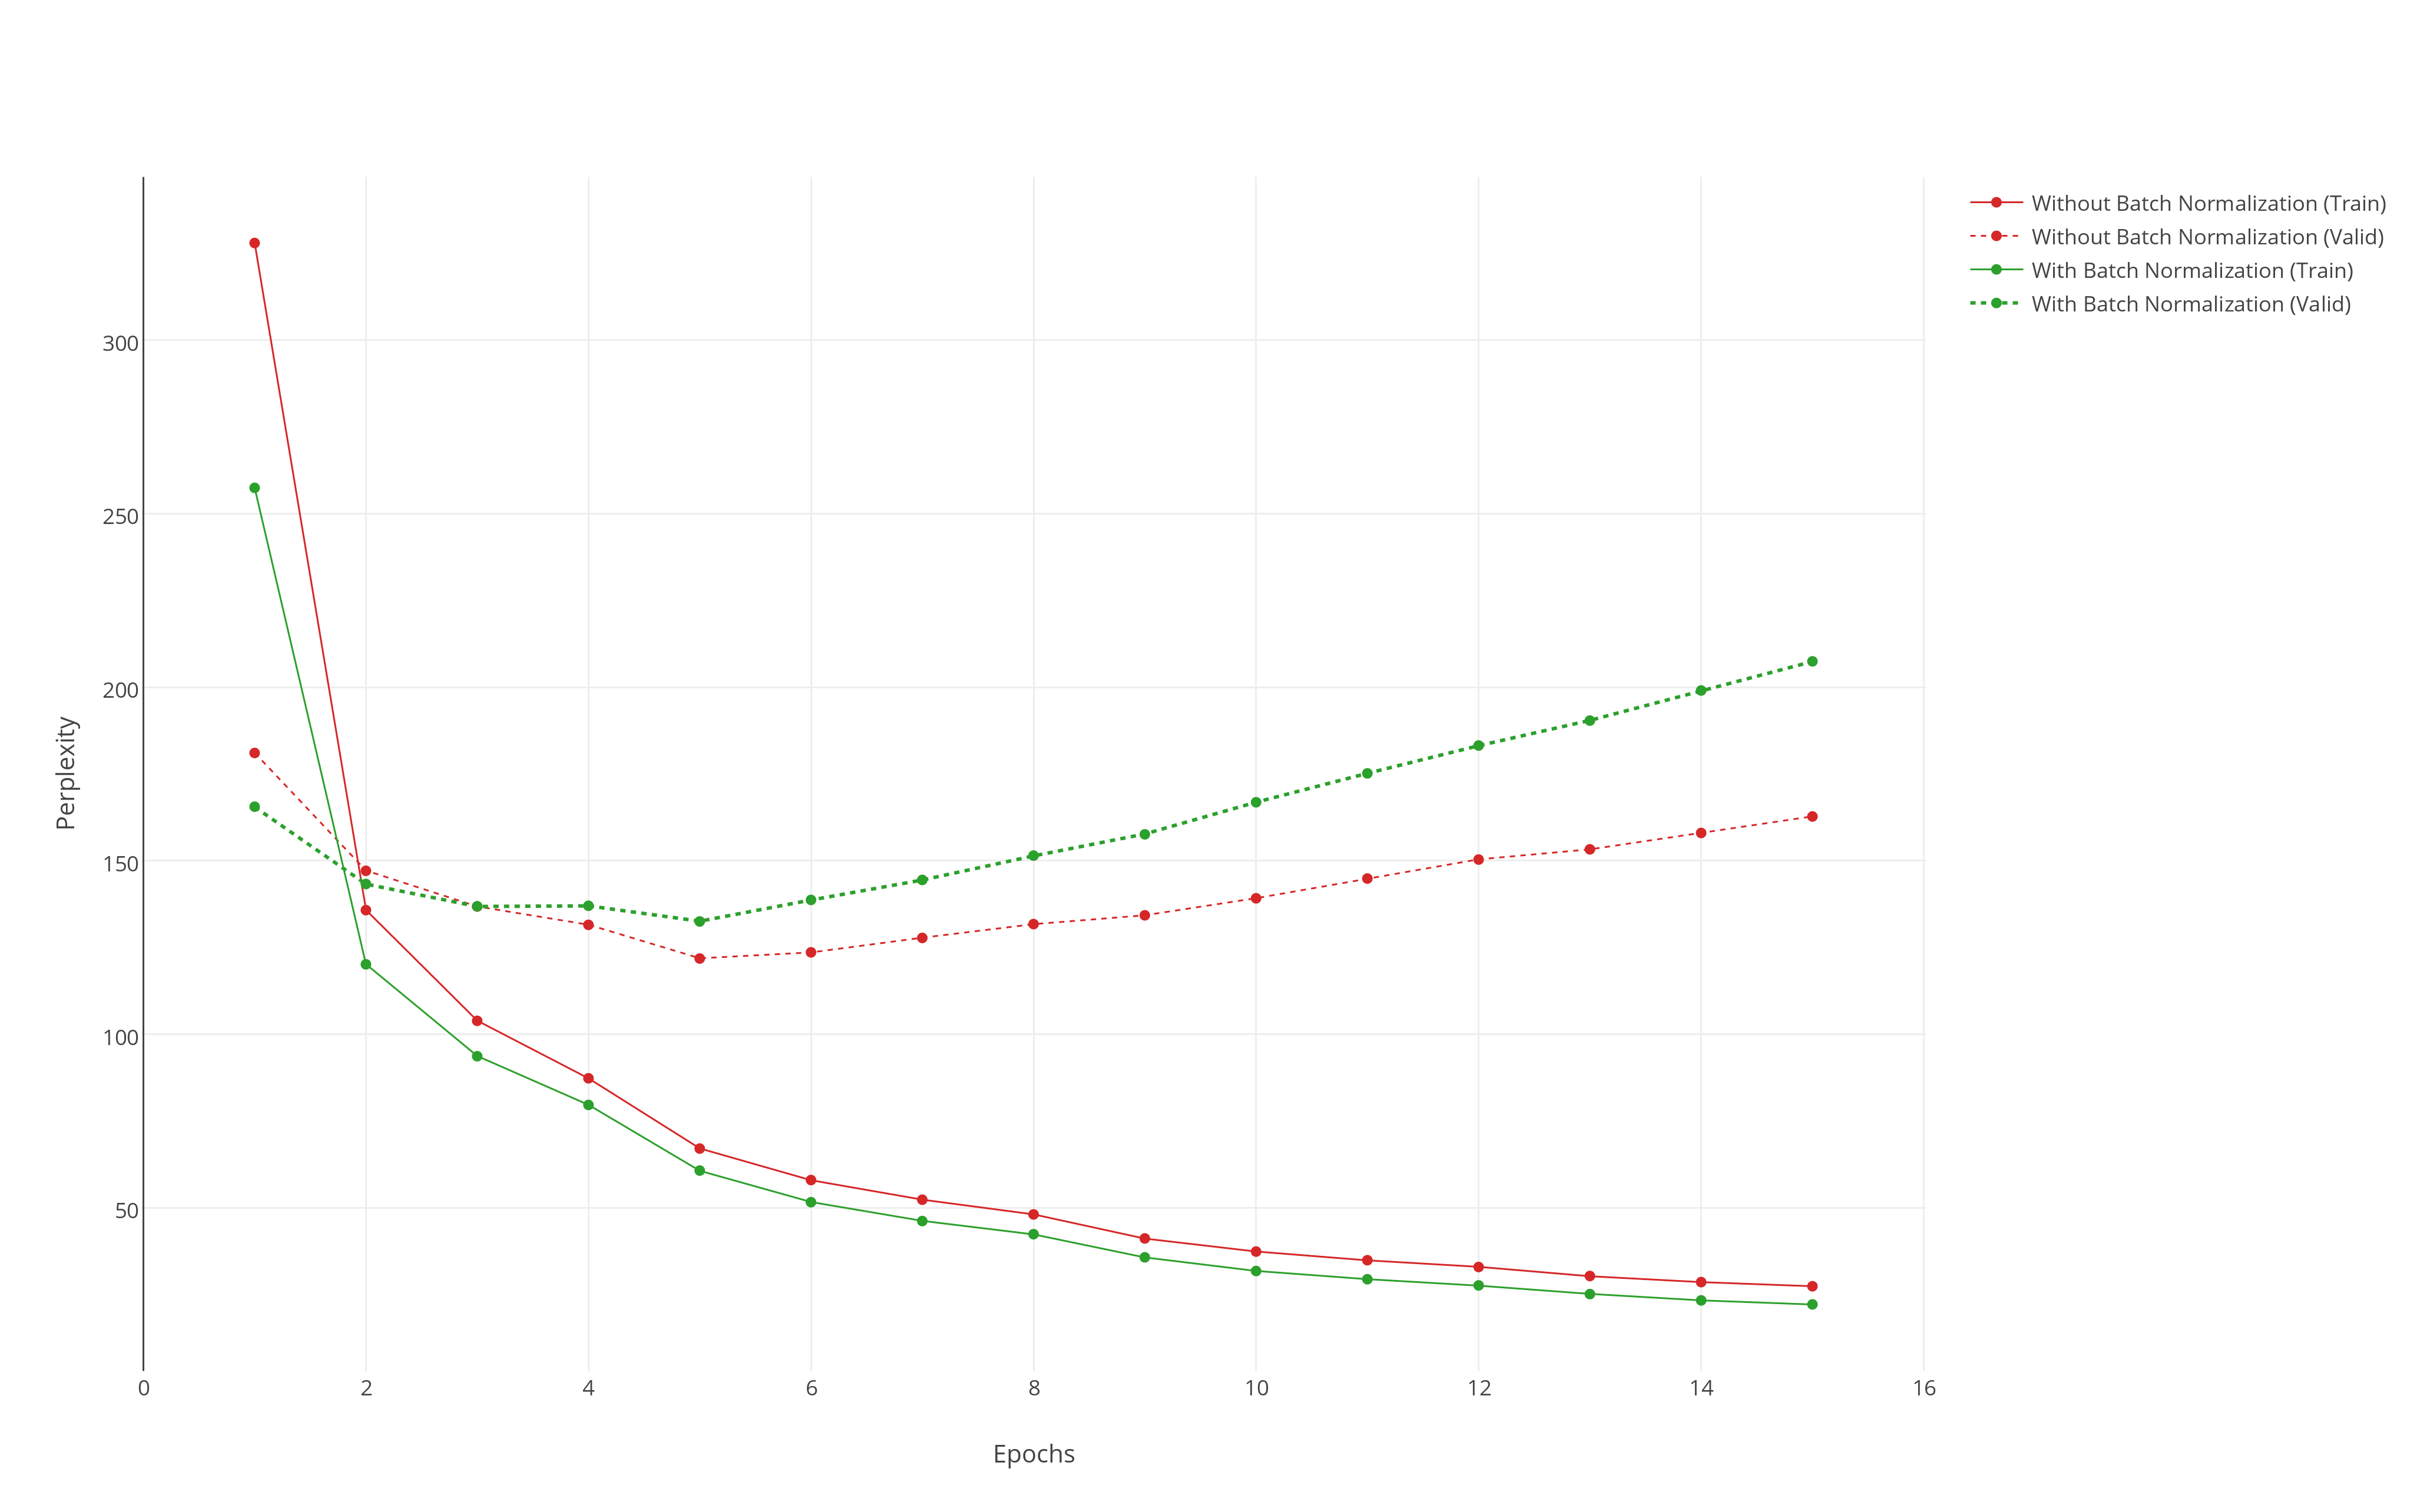
\includegraphics[width=100mm]{ptb_small_norm_plot.png}
  \caption{[Plot iterations instead of epochs, move legend to bottom and make font/lines larger] Small LSTM on Penn Treebank with and without batch normalization.}
  \label{overflow}
\end{figure}


{\renewcommand{\arraystretch}{1.4}

\begin{table}
	\begin{center}
		\begin{tabular}{lcr}
  			\hline
  			
			\multicolumn{1}{l}{\bf Model}  &\multicolumn{1}{c}{\bf Valid Set}  &\multicolumn{1}{c}{\bf Test Set} \\
  			
			\hline
  			
			\multicolumn{3}{c}{Penn Treebank} \\
  			
			\hline

  			Small LSTM		& 120.7 & 114.5 \\
  			Small LSTM (BN)	& 130.0 & 123.9 \\

  			\hline

  			Large LSTM		& 82.2 & \textbf{78.4} \\
  			Large LSTM (BN)	& \\

  			\hline

		\end{tabular}
	
		\caption{[\textit{Bold top and bottom lines}] Word-level perplexity on the Penn Treebank dataset.}

	\end{center}
\end{table}

\subsection{Speech Recognition}

\section{Discussion}

% References should be produced using the bibtex program from suitable
% BiBTeX files (here: strings, refs, manuals). The IEEEbib.bst bibliography
% style file from IEEE produces unsorted bibliography list.
% -------------------------------------------------------------------------
\bibliographystyle{IEEEbib}

%\bibliographystyle{natbib}
\bibliography{paperrefs}

\end{document}
